\documentclass{article}

% PACKAGES for formatting, math, units, and diagrams
\usepackage[a4paper, margin=1in]{geometry}
\usepackage{amsmath}
\usepackage{amssymb}
\usepackage{graphicx}
\usepackage{siunitx}      % For proper formatting of units
\usepackage{tikz}         % For drawing diagrams
\usetikzlibrary{decorations.pathmorphing} % For spring drawing
\usepackage{hyperref}     % For clickable links
\usepackage{amsfonts}
\usepackage{caption}      % For captions in non-floating figures
\usepackage{xcolor}       % For additional color options

% Better equation numbering
\numberwithin{equation}{section}

% SIUNITX setup for consistent formatting
\sisetup{
    per-mode = symbol,
    exponent-product = \cdot,
    tight-spacing = true
}

% DOCUMENT INFORMATION
\title{Electrostatics Lesson Notes \& Olympiad Problem Solutions}
\author{Prepared by Gemini}
\date{\today}

\begin{document}

\maketitle

\section*{Introduction}
This document provides a concise one-hour lesson plan on electrostatics, focusing on the core concepts required to solve several Singapore Physics Olympiad (SPhO) problems. It covers electric fields, potential, Gauss's law, and applications in mechanics. Following the notes, detailed, step-by-step solutions to the provided problems are presented.

\section{Electrostatics Lesson Notes}

\subsection{Electric Fields, Forces, and Potential (\SI{15}{min})}

\subsubsection{Electric Field ($\vec{E}$)}
An electric field is a region around a charged object where another charge experiences a force.
\begin{itemize}
    \item \textbf{Force on a charge:} The electric force $\vec{F}$ on a charge $q$ in an electric field $\vec{E}$ is given by:
    $$ \vec{F} = q\vec{E} $$
    The force on a positive charge is in the direction of $\vec{E}$; the force on a negative charge is opposite to $\vec{E}$.

    \item \textbf{Field from a point charge:} The electric field from a single point charge $Q$ is:
    $$ \vec{E} = \frac{1}{4\pi\epsilon_0} \frac{Q}{r^2} \hat{r} $$
    where $r$ is the distance from the charge and $\epsilon_0 = \SI{8.85e-12}{\farad\per\meter}$ is the permittivity of free space.
\end{itemize}

\subsubsection{Electric Potential ($V$)}
Electric potential is the electric potential energy per unit charge. It's a scalar quantity.
\begin{itemize}
    \item \textbf{Potential from a point charge:}
    $$ V = \frac{1}{4\pi\epsilon_0} \frac{Q}{r} $$
    \item \textbf{Superposition Principle:} The total potential at a point from multiple charges is the algebraic sum of the individual potentials.
    $$ V_{\text{total}} = \sum_{i} V_i = \frac{1}{4\pi\epsilon_0} \sum_{i} \frac{Q_i}{r_i} $$
    \item \textbf{Work and Potential Energy:} The work $W$ required to move a charge $q$ from point B to point A is path-independent:
    $$ W = \Delta U = q\Delta V = q(V_A - V_B) $$
\end{itemize}

\subsection{Continuous Charge Distributions \& Gauss's Law (\SI{20}{min})}
Charge can be spread out over a line, surface, or volume.
\begin{itemize}
    \item Linear charge density $\lambda$ (\si{\coulomb\per\meter})
    \item Surface charge density $\sigma$ (\si{\coulomb\per\meter\squared})
    \item Volume charge density $\rho$ (\si{\coulomb\per\meter\cubed})
\end{itemize}
To find the total effect (force, field, etc.), we integrate. For example, total charge $Q = \int \lambda \,dL$.

\subsubsection{Gauss's Law}
Gauss's Law relates the electric flux through a closed surface (a "Gaussian surface") to the net charge $Q_{\text{enc}}$ enclosed by that surface. It is very useful for symmetric charge distributions.
$$ \oint \vec{E} \cdot d\vec{A} = \frac{Q_{\text{enc}}}{\epsilon_0} $$

\begin{center}
    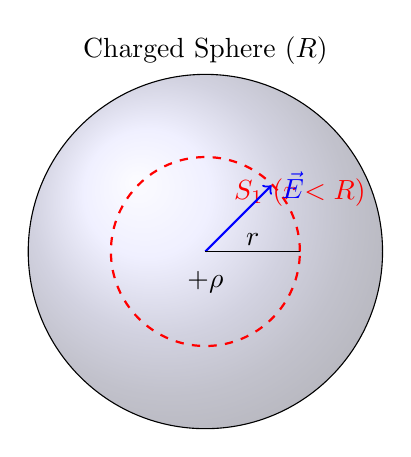
\begin{tikzpicture}[scale=1.5]
        % Sphere
        \shade[ball color=blue!20!white, opacity=0.4] (0,0) circle (1.5);
        \draw (0,0) circle (1.5);
        \node at (0,0) [label=below:{$+\rho$}] {};
        \node at (0, 1.7) {Charged Sphere ($R$)};
        % Gaussian surface inside
        \draw[red, dashed, thick] (0,0) circle (0.8);
        \node[red] at (0.8, 0.5) {$S_1$ ($r<R$)};
        % E-field vector inside
        \draw[->, thick, blue] (0,0) -- (0.56, 0.56) node[right]{$\vec{E}$};
        \draw (0,0) -- (0.8,0);
        \node at (0.4, 0.1) {$r$};
    \end{tikzpicture}
    \captionof{figure}{A spherical Gaussian surface $S_1$ inside a uniformly charged sphere is used to find the E-field at a distance $r < R$.}
\end{center}

\textbf{Key Result: E-field inside a uniformly charged sphere}\\
For a sphere of radius $R$ and uniform charge density $\rho$, the electric field at a distance $r < R$ from the center is:
$$ E = \frac{\rho r}{3\epsilon_0} $$
The force on a particle with charge $-q$ inside is $F = (-q)E = -\frac{q\rho}{3\epsilon_0}r$. This is a restoring force ($F \propto -r$), which leads to Simple Harmonic Motion (SHM).

\subsection{Electrostatics in Mechanics (\SI{25}{min})}
\subsubsection{Static Equilibrium}
For a body to be in equilibrium, two conditions must be met:
\begin{enumerate}
    \item \textbf{Net force is zero:} $\sum \vec{F} = 0$
    \item \textbf{Net torque is zero:} $\sum \vec{\tau} = 0$ (about any pivot)
\end{enumerate}

\subsubsection{Simple Harmonic Motion (SHM)}
SHM occurs when an object experiences a restoring force directly proportional to its displacement from equilibrium: $F = -kx$. This leads to oscillations with an angular frequency $\omega$ and period $T$:
$$ \omega = \sqrt{\frac{k}{m}} \quad \text{and} \quad T = \frac{2\pi}{\omega} $$

\newpage
\section{Olympiad Problem Walkthroughs}

\subsection{Problem 1: Rod in an Electric Field (SPhO 2023)}
\textit{A thin rod AB of length \SI{60}{cm} is suspended by two identical springs ($k=\SI{20}{\newton\per\meter}$) in a uniform downward E-field ($E=\SI{24}{\volt\per\meter}$). The linear charge density is $\lambda = 0.9x$ (in \si{\coulomb\per\meter} with $x$ in \si{\meter}). Find the inclination $\theta$ of the rod.}

\begin{center}
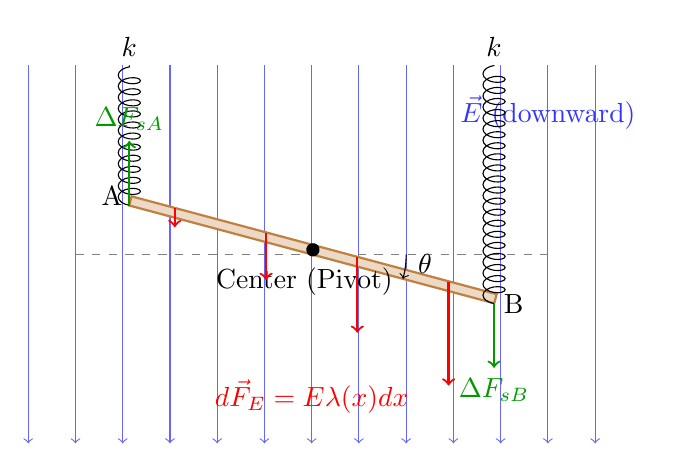
\begin{tikzpicture}[scale=1.2]
    % Electric field
    \foreach \x in {-3,-2.5,...,3} {
        \draw[->, blue!60, thin] (\x, 2) -- (\x, -2);
    }
    \node[blue!80] at (2.5, 1.5) {$\vec{E}$ (downward)};
    % Horizontal reference line
    \draw[dashed, gray] (-2.5, 0) -- (2.5, 0);
    % Tilted rod
    \begin{scope}[rotate=-15]
        \draw[thick, brown, fill=brown!30] (-2, 0) rectangle (2, 0.1);
        \node at (-2.2, 0.05) {A};
        \node at (2.2, 0.05) {B};
        \node at (0, -0.3) {Center (Pivot)};
        \fill (0, 0.05) circle (2pt);
    \end{scope}
    % Angle theta
    \draw[->] (1,0) arc (0:-15:1);
    \node at (1.2, -0.1) {$\theta$};
    % Springs
    \draw[decoration={coil,aspect=0.5,segment length=4pt,amplitude=4pt},decorate] (-1.93, 0.52) -- (-1.93, 2);
    \node at (-1.93, 2.2) {$k$};
    \draw[decoration={coil,aspect=0.5,segment length=4pt,amplitude=4pt},decorate] (1.93, -0.52) -- (1.93, 2);
    \node at (1.93, 2.2) {$k$};
    % Forces
    \draw[->, thick, green!60!black] (-1.93, 0.52) -- (-1.93, 1.2) node[above] {$\Delta F_{sA}$};
    \draw[->, thick, green!60!black] (1.93, -0.52) -- (1.93, -1.2) node[below] {$\Delta F_{sB}$};
    % Electric Force (non-uniform)
    \foreach \x in {-1.5, -0.5, 0.5, 1.5} {
        \pgfmathsetmacro{\force}{0.2 + 0.3*(\x+1.5)}
        \pgfmathsetmacro{\xcoord}{\x*cos(-15)}
        \pgfmathsetmacro{\ycoord}{\x*sin(-15)+0.1}
        \draw[->, thick, red] (\xcoord, \ycoord) -- (\xcoord, \ycoord-\force);
    }
    \node[red] at (0, -1.5) {$d\vec{F}_E = E\lambda(x)dx$};
\end{tikzpicture}
\captionof{figure}{Free-body diagram for the tilted rod in equilibrium.}
\end{center}

\textbf{Solution Strategy:} We balance the torques about the center of the rod.
\begin{enumerate}
    \item \textbf{Electric Torque ($\tau_E$):}
    \begin{align*}
        \tau_E = \int_0^L (x - L/2) (E \lambda(x) \cos\theta) \,dx = 21.6 \cos\theta \frac{L^3}{12}
    \end{align*}
    With $L = \SI{0.60}{m}$, $\tau_E = 0.3888 \cos\theta$ (clockwise).

    \item \textbf{Spring Torque ($\tau_S$):}
    $$ \tau_S = k \frac{L^2}{2} \sin\theta \cos\theta $$
    With $k=\SI{20}{\newton\per\meter}$ and $L = \SI{0.60}{m}$, $\tau_S = 3.6 \sin\theta \cos\theta$ (counter-clockwise).

    \item \textbf{Equilibrium:} Set $\tau_E = \tau_S$:
    \begin{align*}
        0.3888 \cos\theta = 3.6 \sin\theta \cos\theta \implies \sin\theta = \frac{0.3888}{3.6} = 0.108 \implies \theta \approx \SI{6.2}{\degree}
    \end{align*}
\end{enumerate}

\hrulefill
\subsection{Problem 2: Point Charges in a Rectangle (SPhO 2021)}
\textit{A rectangle has sides \SI{5.0}{cm} and \SI{15}{cm}. Arrangement: $q_1 = \SI{-5.0}{\micro\coulomb}$ (top left), A (top right), B (bottom left), $q_2 = \SI{+2.0}{\micro\coulomb}$ (bottom right).}

\begin{center}
    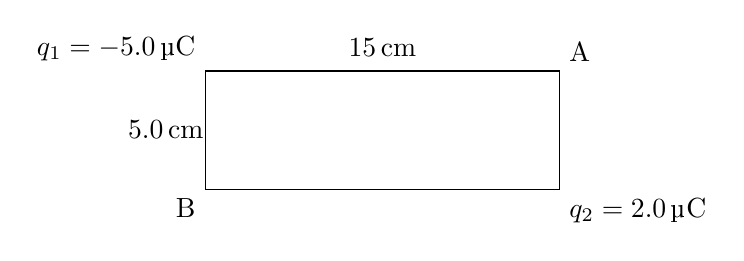
\begin{tikzpicture}
        \draw (0,1.5) -- (4.5,1.5) -- (4.5,0) -- (0,0) -- (0,1.5);
        \node at (0,1.5) [above left] {$q_1=\SI{-5.0}{\micro\coulomb}$};
        \node at (4.5,1.5) [above right] {A};
        \node at (0,0) [below left] {B};
        \node at (4.5,0) [below right] {$q_2=\SI{+2.0}{\micro\coulomb}$};
        \node at (2.25, 1.8) {\SI{15}{cm}};
        \node at (-0.5, 0.75) {\SI{5.0}{cm}};
    \end{tikzpicture}
    \captionof{figure}{The corrected arrangement of charges and points.}
\end{center}

Let $k = \dfrac{1}{4\pi\epsilon_0} \approx \SI{9.0e9}{\newton\meter\squared\per\coulomb\squared}$.

\begin{enumerate}
    \item[(a)] \textbf{Potential at corner A:} $r_{1A} = \SI{0.15}{m}$, $r_{2A} = \SI{0.05}{m}$.
    \begin{align*}
        V_A &= (\SI{9.0e9}{\newton\meter\squared\per\coulomb\squared}) \left( \frac{\num{-5.0e-6}}{\SI{0.150}{\meter}} + \frac{\num{2.0e-6}}{\SI{0.050}{\meter}} \right) \si{\coulomb} \\
        &= \SI{9.0e9}{} \left( -3.333\times10^{-5} + 4.000\times10^{-5} \right) \si{\volt} \\
        &= \SI{+6.00e4}{\volt}
    \end{align*}

    \item[(b)] \textbf{Potential at corner B:} $r_{1B} = \SI{0.05}{m}$, $r_{2B} = \SI{0.15}{m}$.
    \begin{align*}
        V_B &= (\SI{9.0e9}{\newton\meter\squared\per\coulomb\squared}) \left( \frac{\num{-5.0e-6}}{\SI{0.050}{\meter}} + \frac{\num{2.0e-6}}{\SI{0.150}{\meter}} \right) \si{\coulomb} \\
        &= \SI{9.0e9}{} \left( -1.000\times10^{-4} + 1.333\times10^{-5} \right) \si{\volt} \\
        &= \SI{-7.80e5}{\volt}
    \end{align*}

    \item[(c)] \textbf{Work to move $q_3 = \SI{+3.0}{\micro\coulomb}$ from B to A:}
    \begin{align*}
        W_{B \to A} &= q_3 (V_A - V_B) \\
        &= (\SI{3.0e-6}{\coulomb}) (\SI{+6.00e4}{\volt} - (\SI{-7.80e5}{\volt})) \\
        &= (\SI{3.0e-6}{\coulomb}) (\SI{8.40e5}{\volt}) = \SI{+2.52}{\joule}
    \end{align*}

    \item[(d)] The work done by the external agent is positive. This means the system's electric potential energy \textbf{increases}.
    
    \item[(e) \& (f)] The electrostatic force is conservative. Therefore, the work done is \textbf{the same} because it is path-independent.
\end{enumerate}

\hrulefill
\subsection{Problem 3: Merging Oil Drops (SPhO 2019)}
\textit{Two identical spherical oil drops with surface potential \SI{1000}{V} unite to form a single drop. What is the potential of the new drop?}

\begin{enumerate}
    \item \textbf{Initial State:} For one drop with charge $Q_1$ and radius $R_1$:
    $$ V_1 = \frac{k Q_1}{R_1} = \SI{1000}{V} $$
    
    \item \textbf{Conservation Laws:} When the drops merge:
    \begin{itemize}
        \item New charge: $Q_2 = 2Q_1$
        \item New volume: $V_{\text{vol,2}} = 2 V_{\text{vol,1}}$
    \end{itemize}
    
    \item \textbf{Find New Radius ($R_2$):}
    \begin{align*}
        \frac{4}{3}\pi R_2^3 &= 2 \times \frac{4}{3}\pi R_1^3 \\
        R_2^3 &= 2 R_1^3 \implies R_2 = 2^{1/3} R_1
    \end{align*}

    \item \textbf{Calculate New Potential ($V_2$):}
    \begin{align*}
        V_2 &= \frac{k Q_2}{R_2} = \frac{k(2Q_1)}{2^{1/3}R_1} = 2^{2/3} \left( \frac{kQ_1}{R_1} \right) \\
        V_2 &= 2^{2/3} V_1 = 2^{2/3} (\SI{1000}{V}) \approx \num{1.5874} \times \SI{1000}{V} = \SI{1587}{V}
    \end{align*}
\end{enumerate}

\hrulefill
\subsection{Problem 4: Particle in a Sphere Tunnel (SPhO 2020 \& 2023)}
\textit{A particle ($m$, $-q$) is released in a tunnel through a sphere (radius $R$, density $\rho$).}

\begin{enumerate}
    \item \textbf{Equation of Motion:} The E-field inside the sphere at distance $r$ is $E = \dfrac{\rho r}{3\epsilon_0}$. The force on charge $-q$ is:
    $$ F = (-q)E = -\left(\frac{q\rho}{3\epsilon_0}\right)r $$
    This is SHM, where the effective spring constant is $k_{\text{eff}} = \dfrac{q\rho}{3\epsilon_0}$.
    
    \item \textbf{Description of Motion:} The particle undergoes \textbf{Simple Harmonic Motion (SHM)} about the center of the sphere with an amplitude of $R$.
    
    \item \textbf{Calculations (SPhO 2023):}
    
    Given: $R=\SI{0.50}{m}$, $\rho = \SI{5.0}{\nano\coulomb\per\meter\cubed} = \SI{5.0e-9}{\coulomb\per\meter\cubed}$, $m=\SI{1.0}{\micro\gram} = \SI{1.0e-9}{kg}$, $q = \SI{0.05}{\nano\coulomb} = \SI{5.0e-11}{C}$.
    \begin{itemize}
        \item Angular frequency:
        \begin{align*}
            \omega &= \sqrt{\frac{q\rho}{3\epsilon_0 m}} \\
            &= \sqrt{\frac{(\num{5.0e-11})(\num{5.0e-9})}{3(\num{8.85e-12})(\num{1.0e-9})}} \\
            &\approx \sqrt{9.416} \approx \SI{3.07}{\radian\per\second}
        \end{align*}
        \item Time to cross the tunnel is half a period ($T/2$):
        $$ T = \frac{2\pi}{\omega} \approx \SI{2.05}{s} \implies t = \frac{T}{2} \approx \SI{1.02}{s} $$
        \item Speed at the center is the maximum speed in SHM ($v_{\text{max}} = A\omega$):
        $$ v_{\text{center}} = R\omega = (\SI{0.50}{m})(\SI{3.07}{\radian\per\second}) \approx \SI{1.54}{\meter\per\second} $$
    \end{itemize}
    \item \textbf{Speed Calculation (SPhO 2020):} In terms of variables, the speed is:
    $$ v_{\text{center}} = R\sqrt{\frac{q\rho}{3\epsilon_0 m}} $$
\end{enumerate}

\hrulefill
\subsection{Problem 5: Charged Object on Ring Axis (SPhO 2022)}
\textit{A ring ($R=\SI{50}{cm}, \lambda = \SI{+10}{\nano\coulomb\per\meter}$) and an object ($m=\SI{1}{mg}, q=\SI{-5.0}{\nano\coulomb}$) starting at $x_0 = \SI{5.0}{mm}$.}

\begin{enumerate}
    \item \textbf{Approximation for SHM:} The E-field on the axis is $E_x = \dfrac{kQx}{(R^2+x^2)^{3/2}}$.
    Since $x_0 \ll R$, we approximate $(R^2+x^2)^{3/2} \approx R^3$.
    $$ E_x \approx \frac{kQ}{R^3}x $$
    The force on charge $q$ is $F_x = qE_x \approx -\frac{k|q|Q}{R^3}x$. This is SHM with $k_{\text{eff}} = \dfrac{k|q|Q}{R^3}$.
    
    \item[(a)] \textbf{Time to reach the center:} This time is one-quarter of a period ($T/4$).
    \begin{itemize}
        \item Total charge on ring: $Q = \lambda(2\pi R) = (\SI{10e-9}{\coulomb\per\meter})(2\pi \times \SI{0.50}{m}) = \num{3.142e-8} \si{\coulomb}$.
        \item Effective spring constant:
        \begin{align*}
            k_{\text{eff}} &= \frac{(\num{9.0e9})(\num{5.0e-9})(\num{3.142e-8})}{(\num{0.50})^3} \\
            &= \frac{\num{1.414e-6}}{0.125} \approx \SI{1.131e-5}{\newton\per\meter}
        \end{align*}
        \item Angular frequency: $\omega = \sqrt{\frac{k_{\text{eff}}}{m}} = \sqrt{\frac{\SI{1.131e-5}{\newton\per\meter}}{\SI{1.0e-6}{kg}}} \approx \SI{3.36}{\radian\per\second}$.
        \item Period: $T = \frac{2\pi}{\omega} \approx \SI{1.87}{s}$.
        \item Time to center: $t = T/4 \approx \SI{0.468}{s}$.
    \end{itemize}

    \item[(b)] \textbf{Kinetic Energy at the center:} Use conservation of energy. $K_f = -q(V(0) - V(x_0))$.
    The potential on the axis is $V(x) = \dfrac{kQ}{\sqrt{R^2+x^2}}$.
    \begin{align*}
        K_f &= -q \left( \frac{kQ}{R} - \frac{kQ}{\sqrt{R^2+x^2}} \right) \\
        &= (\SI{5.0e-9}{\coulomb}) \cdot (\num{9.0e9}) \cdot (\num{3.142e-8}) \left( \frac{1}{0.50} - \frac{1}{\sqrt{0.50^2 + 0.005^2}} \right) \\
        &= (\num{1.414e-6}) \left( 2.0000 - 1.9999 \right) \approx \SI{1.41e-10}{\joule}
    \end{align*}
\end{enumerate}

\newpage
\section{Derivations of Key Formulas}

\subsection{Derivation for Problem 4: E-Field Inside a Uniform Sphere}
The electric field inside a uniformly charged sphere is found using \textbf{Gauss's Law}, which works perfectly for symmetric charge distributions.

\textbf{1. The Setup:}
\begin{itemize}
    \item We have a sphere of radius $R$ with a uniform volume charge density $\rho$.
    \item We want to find the electric field $E$ at a distance $r$ from the center, where $r < R$.
    \item Due to the spherical symmetry, the electric field must point radially outward and its magnitude can only depend on the distance $r$.
\end{itemize}

\textbf{2. Applying Gauss's Law:}
Gauss's Law is $\oint \vec{E} \cdot d\vec{A} = \frac{Q_{\text{enc}}}{\epsilon_0}$.
\begin{itemize}
    \item \textbf{Gaussian Surface:} We choose a smaller, imaginary sphere of radius $r$ inside the larger sphere. This is our Gaussian surface.
    \item \textbf{Left Side (Flux Integral):} On this surface, the electric field $\vec{E}$ is always parallel to the area vector $d\vec{A}$. So, $\vec{E} \cdot d\vec{A} = E \, dA$. Since $E$ is constant at a given $r$, the integral becomes:
    $$ \oint E \, dA = E \oint dA = E (\text{Surface Area of Gaussian Sphere}) = E (4\pi r^2) $$
    \item \textbf{Right Side (Enclosed Charge):} We need the charge $Q_{\text{enc}}$ inside our Gaussian sphere of radius $r$.
    $$ Q_{\text{enc}} = \text{Density} \times \text{Volume} = \rho \times V_{\text{Gaussian}} = \rho \left( \frac{4}{3}\pi r^3 \right) $$
\end{itemize}

\textbf{3. Solving for E:}
Now we set the left and right sides of Gauss's Law equal:
\begin{align*}
    E (4\pi r^2) &= \frac{1}{\epsilon_0} \left( \rho \frac{4}{3}\pi r^3 \right) \\
    E &= \frac{\rho \frac{4}{3}\pi r^3}{\epsilon_0 (4\pi r^2)} \\
    E &= \frac{\rho r}{3\epsilon_0}
\end{align*}
This is the required formula. It shows that the electric field inside the sphere increases linearly with the distance from the center.

\subsection{Derivation for Problem 5: E-Field on the Axis of a Charged Ring}
For charge distributions that are not highly symmetric (like a ring), we must integrate the contributions from each small piece of charge using \textbf{Coulomb's Law}.

\textbf{1. The Setup:}
\begin{itemize}
    \item We have a ring of radius $R$ with a total charge $Q$ distributed uniformly.
    \item We want to find the E-field at a point P on the axis, a distance $x$ from the center.
    \item Consider a small element of charge $dQ$ on the ring.
\end{itemize}

\begin{center}
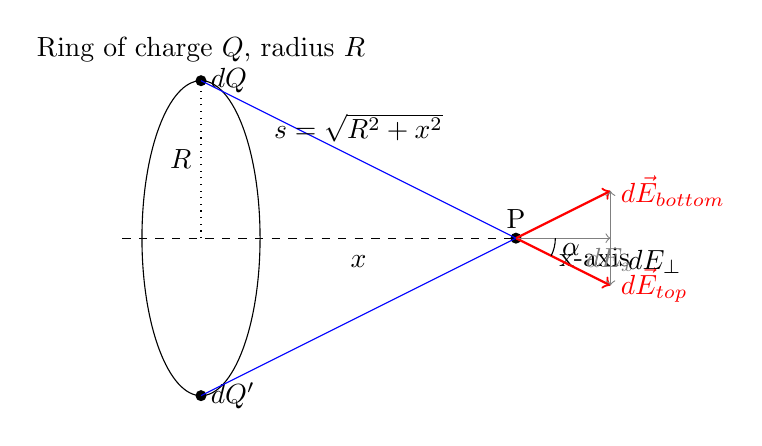
\begin{tikzpicture}
    % Ring in vertical plane
    \draw (0,0) ellipse (0.75cm and 2cm);
    \node at (0, 2.4) {Ring of charge $Q$, radius $R$};
    
    % Axis
    \draw[dashed] (-1,0) -- (5,0) node[below] {x-axis};
    
    % Point P
    \fill (4,0) circle (2pt) node[above] {P};
    \node at (2, -0.3) {$x$};
    
    % Charge element dQ at top
    \fill (0,2) circle (2pt) node[right] {$dQ$};
    
    % Line from dQ to P
    \draw[blue] (0,2) -- (4,0);
    \node at (2,1.4) {$s = \sqrt{R^2+x^2}$};
    
    % Radius R
    \draw[dotted] (0,0) -- (0,2) node[midway, left] {$R$};
    
    % dE vector from top element
    \draw[->, thick, red] (4,0) -- (5.2, -0.6) node[anchor=west] {$d\vec{E}_{top}$};
    
    % dE_x component
    \draw[->, gray] (4,0) -- (5.2,0) node[below] {$dE_x$};
    
    % dE_perp component (downwards)
    \draw[->, gray] (5.2,0) -- (5.2, -0.6);
    \node at (5.3, -0.3) [right] {$dE_\perp$};
    
    % Charge element dQ at bottom
    \fill (0,-2) circle (2pt) node[right] {$dQ'$};
    \draw[blue] (0,-2) -- (4,0);
    
    % dE vector from bottom element
    \draw[->, thick, red] (4,0) -- (5.2, 0.6) node[anchor=west] {$d\vec{E}_{bottom}$};
    
    % dE_perp component (upwards) - cancels the other one
    \draw[->, gray] (5.2,0) -- (5.2, 0.6);
    
    % Angle alpha
    \begin{scope}[shift={(4,0)}]
        \draw (0,0) ++ (0.5,0) arc (0:-26.5:0.5);
        \node at (0.7,-0.15) {$\alpha$};
    \end{scope}
\end{tikzpicture}
\captionof{figure}{A ring in the vertical plane. The perpendicular components ($dE_\perp$) from opposite charge elements ($dQ$ and $dQ'$) cancel out at point P, leaving only the axial components ($dE_x$).}
\end{center}

\textbf{2. Symmetry Argument:}
The electric field $d\vec{E}$ from the charge element $dQ$ has a component along the x-axis ($dE_x$) and a component perpendicular to it ($dE_\perp$). For every $dQ$ at the top of the ring, there is another $dQ$ at the bottom. The perpendicular components from these two elements will point in opposite directions and cancel each other out. This is true for all pairs of opposite points. Therefore, only the x-components of the electric field add up.

\textbf{3. Integrating the x-component:}
\begin{itemize}
    \item The magnitude of the field from $dQ$ is $dE = \frac{k \, dQ}{s^2} = \frac{k \, dQ}{R^2 + x^2}$.
    \item The x-component is $dE_x = dE \cos\alpha$. From the diagram's geometry, $\cos\alpha = \frac{x}{s} = \frac{x}{\sqrt{R^2+x^2}}$.
    \item Combining these, we get:
    $$ dE_x = \left( \frac{k \, dQ}{R^2 + x^2} \right) \left( \frac{x}{\sqrt{R^2+x^2}} \right) = \frac{k x \, dQ}{(R^2+x^2)^{3/2}} $$
\end{itemize}

\textbf{4. Solving for E$_x$:}
To find the total field, we integrate $dE_x$ around the entire ring.
$$ E_x = \int_{\text{ring}} dE_x = \int \frac{k x \, dQ}{(R^2+x^2)^{3/2}} $$
For every charge element $dQ$ on the ring, the terms $k, x,$ and $R$ are constant. So we can pull them out of the integral:
$$ E_x = \frac{k x}{(R^2+x^2)^{3/2}} \int dQ $$
The integral of all the charge elements, $\int dQ$, is simply the total charge of the ring, $Q$.
$$ E_x = \frac{k Q x}{(R^2+x^2)^{3/2}} $$
Since the field is only in the x-direction, this is the total electric field vector, which matches the formula provided in the problem.

\end{document}